% !TeX encoding = UTF-8
% !TeX spellcheck = cs_CZ
% !TeX root = PrezentaceBeamer.tex
\documentclass[hyperref={unicode}]{beamer}

\mode<presentation>
{
	\usetheme{CambridgeUS}
	\setbeamercovered{transparent}
}

\usepackage[czech]{babel}
\usepackage{palatino}
\usepackage{graphicx}

\usepackage{amsmath}
\usepackage{centernot}

\usepackage[utf8]{inputenc}

% Z těchto informací se vygeneruje úvodní stránka
\title{Obecné rotační NURBS plochy}
\subtitle{NURBS surface of revolution}
\author{Ondřej Sekáč}
\institute[ÚM FSI VUT v Brně]{
\includegraphics[width=6cm]{obrazky/ustav.png}}
\date{19. 2. 2018}

\begin{document}
	
	\begin{frame}
	\titlepage
	\begin{center}
		Vedoucí práce: Mgr. Jana Procházková, Ph.D.
	\end{center}
\end{frame}

\begin{frame}{}
\tableofcontents
\end{frame}

\section{Cíle}

\begin{frame}
\frametitle{Cíle}

%  \begin{block}{Motivace}
%  	\begin{itemize}
%  		\item 
%  		\item 
%  		\item 
%  	\end{itemize}
%  \end{block}

\begin{block}{Cíle, kterých má být dosaženo}
\begin{enumerate}
	\item Shrnutí základních teoretických poznatků.
	\item Vytvoření programu obecných rotačních NURBS ploch.
	\item Zobrazení výsledků.
\end{enumerate}
\end{block}
\end{frame}

\section{Úvod do křivek}

\begin{frame}{Úvod do křivek}
Je-li $M$ prostor (např. Eukleidovský) a $I$ interval reálných čísel, pak křivkou $k$ rozumíme spojité zobrazení z $I$ do $M$.
\\\medskip
Někdy se slovem křivka myslí pouze její obraz, tj. množina $K=\{k(x);x\in I\}$.
\\\medskip
\begin{block}{Křivky v počítačové grafice}
Většinou je dána množina řídících bodů (řídící polygon) a matematický aparát, který z jejich polohy určí průběh křivky.
\\\medskip
Popis pomocí polynomů - snadné výpočty, jednoduchá diferencovatelnost.
\end{block}
\end{frame}

% \begin{frame}{Rozdělení křivek}
% \begin{itemize}
% \item Bézierovy křivky
% \begin{itemize}
% \item Racionální Bézierovy křivky
% \end{itemize}
% \item B-spline křivky
% \begin{itemize}
% \item NURBS - Neuniformní racionální B-spline křivky
% \end{itemize}
% \end{itemize}

% \begin{center}
%     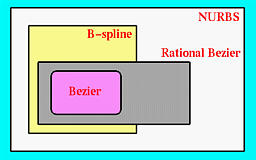
\includegraphics[width=6cm]{obrazky/hierarchy.jpg}
%   \end{center}
% \end{frame}

% \subsection{Bézierovy křivky}
% \begin{frame}{Bézierovy křivky}
% Beziérova křivka stupně $n$ určená řídícím polygonem $P_{0},...,P_{n}$ je dána vztahem
% $$C\left(t\right)=\sum _{i=0}^{n}{B}_{n,i}\left(t\right){P}_{i},\quad t\in\left\langle 0;1 \right\rangle$$
% kde ${B}_{n,i}(t)$ jsou tzv. Bernsteinovy polynomy stupně n
% $$B_{n,i}(t)=\frac{n!}{i!(n-i)!}t^i(1-t)^{n-i}$$
% De Casteljau algoritmus - opakovaná lineární interpolace všech dvojic po sobě jdoucích bodů
% \begin{center}
% 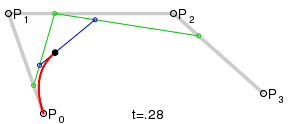
\includegraphics[width=6cm]{obrazky/bezier1.png}
% 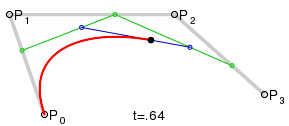
\includegraphics[width=6cm]{obrazky/bezier2.png}
% \end{center}
% \end{frame}

% \subsubsection{Racionální Bézierovy křivky}
% \begin{frame}{Racionální Bézierovy křivky}
% Některé objekty (části kružnic) nelze popsat pomocí Bézierových křivek, protože je nelze popsat polynomiální parametrizací a je potřeba použít racionální lomené funkce. Využíváme tzv.
% \begin{block}{Homogenní souřadnice}
% Bod $P=\left[x,y,z\right]$ má homogenní souřadnice $P_w=\left[wx,wy,wz,w\right]$ pro $w\neq0$. Souřadnici $w$ nazýváme váhou bodu P.
% \end{block}
% Parametrizaci racionální Bézierovy křivky poté získáme ze vztahu
% $$C_{w}\left(t\right)=\sum _{i=0}^{n}{B}_{n,i}\left(t\right){P}_{w_i} \implies C\left(t\right)=\frac{\sum _{i=0}^{n}{B}_{n,i}\left(t\right)w_i{P}_{i}}{\sum _{i=0}^{n}{B}_{n,i}\left(t\right)w_i},\quad t\in\left\langle 0;1 \right\rangle$$
% \end{frame}

% \begin{frame}
% \begin{center}
% 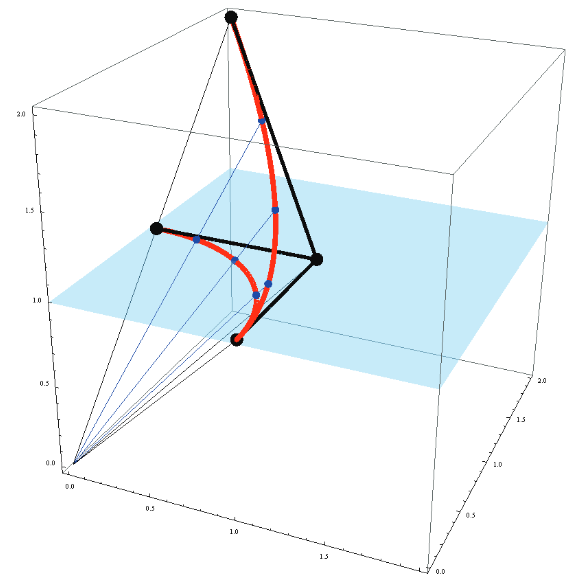
\includegraphics[width=6cm]{obrazky/projection.png}
% \end{center}
% \end{frame}

\subsection{B-spline křivky}
\begin{frame}{B-spline křivky}
%Podobně jako Bézierova křivka, je 
B-spline křivka stupně $n$ určená řídícími body $P_0,...,P_n$ je dána vztahem
$$C\left(u\right)=\sum _{i=0}^{n}{N}_{i,p}\left(u\right){P}_{i},\quad u\in U$$
kde $U$ je neklesající posloupnost $\left(m+1\right)$ reálných čísel $u_0\leq u_1\leq ... \leq u_m$, kterou nazýváme uzlový vektor\footnote{Většinou budeme uvažovat $u_0=0$ a $u_m=1$, tedy $U=\left\langle 0;1\right\rangle$.\\}. Čísla $u_i$ nazýváme uzly a interval $\left\langle u_i;u_{i+1}\right)$ $i$-tou uzlovou roztečí.
\\\medskip
Je-li hodnota výrazu $u_{i+1}-u_i$ konstantní pro všechna $i=0,1,...,m-1$, označujeme uzlový vektor jako uniformní, jinak hovoříme o neuniformním uzlovém vektoru.
\end{frame}

\begin{frame}{B-spline bázové funkce}
Na daném uzlovém vektoru $U=\left\langle u_0;u_m\right\rangle$ jsou pro $i=0,...,n$ B-spline bázové funkce definovány rekurentně pomocí tzv. Cox-de Boorovy formule
$$N_{i,0}(u)=\left\{\begin{matrix}1 & u\in\left\langle u_i;u_{i+1} \right)
\\ 
0 & jinak
\end{matrix}\right.$$
$$N_{i,p}(u)=\frac{u-u_i}{u_{i+p}-u_i}N_{i,k-p}(u)+\frac{u_{i+p+1}-u}{u_{i+p+1}-u_{i+1}}N_{i+1,p-1}(u)$$
kde $p=m-n-1$ nazýváme stupeň bázové funkce (resp. křivky).
\end{frame}

\begin{frame}{Dvě důležité vlastnosti}
% \begin{center}
% $N_{i,0}(u)=\left\{\begin{matrix}1 & u\in\left\langle u_i;u_{i+1} \right)
% \\ 
% 0 & jinak
% \end{matrix}\right.$
% $N_{i,p}(u)=\frac{u-u_i}{u_{i+p}-u_i}N_{i,k-p}(u)+\frac{u_{i+p+1}-u}{u_{i+p+1}-u_{i+1}}N_{i+1,p-1}(u)$
% \\\medskip
% 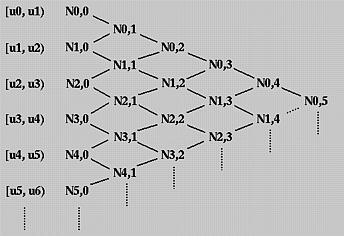
\includegraphics[width=5cm]{obrazky/bs-scheme.jpg}
% \\\medskip
% \end{center}

\begin{minipage}{0.4\textwidth}
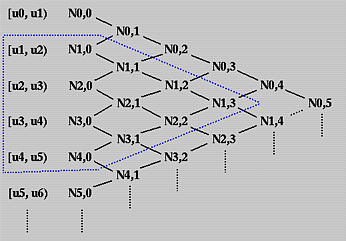
\includegraphics[width=\linewidth]{obrazky/bs-back.jpg}
\end{minipage}
\begin{minipage}{0.55\textwidth}\raggedright
Bázová funkce $N_{i,p}\left(u\right)$ je nenulová na intervalu $\left\langle u_i;u_{i+p+1} \right) \implies$ je nenulová na $p+1$ uzlových roztečích
\end{minipage}
\\\medskip
\begin{minipage}{0.4\textwidth}
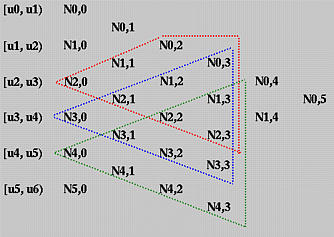
\includegraphics[width=\linewidth]{obrazky/bs-non-0.jpg}
\end{minipage}
\begin{minipage}{0.55\textwidth}\raggedright
Na každé rozteči uzlového vektoru je nejvýše $p+1$ racionálních bázových funkcí nenulových.\\
$N_{i-p,p},N_{i-p+1,p},...N_{i,p}$
\end{minipage}
\end{frame}

\begin{frame}{DeBoorův algoritmus}
Zvyšováním násobnosti uzlů se snižuje počet nenulových bázových funkcí na tomto uzlu. Pokud je uzel násobnosti $p$, existuje pouze jediná nenulová bázová funkce, rovna jedné. Dostáváme tedy
$$C\left(u\right)=N_{i,p}\left(u\right)P_i=P_i$$
Budeme tedy opakovaně vkládat uzel $u$, dokud se nestane $p$-násobným. Vkládání se provádí lineární interpolací dle
$$P_{i,r}=\left(1-a_{i,r}\right)P_{i-1,r-1}+a_{i,r}P_{i,r-1},\quad kde$$
$$a_{i,r}=\frac{u-u_i}{u_{i+p-r+1}-u_i}$$
pro $u\in \left\langle u_k;u_{u_k+1}\right)$, $r=1,...,p$ a $i=k-p+r,...,k$
\end{frame}

\subsection{NURBS - Neuniformní racionální B-spline křivky}
\begin{frame}{NURBS - Neuniformní racionální B-spline křivky}
%Stejně jako u Bézierových křivek, zavedeme homogenní souřadnice i pro B-spline křivky.
Některé objekty nelze popsat polynomiální parametrizací a je potřeba použít racionální lomené funkce. K zobrazení kružnic a dalších kuželoseček, ale také jako další prvek pro ovladatelnost tvaru křivky využíváme tzv.
\begin{block}{Homogenní souřadnice}
Bod $P=\left[x,y,z\right]$ má homogenní souřadnice $P_w=\left[wx,wy,wz,w\right]$ pro $w\neq0$. Souřadnici $w$ nazýváme váhou bodu P.
\end{block}
Pro řídící body $P_0,...,P_n$, kterým jsou přiřazeny nezáporné váhy $\left\lbrace w_0,...,w_n \right\rbrace$ a uzlový vektor $U=\left\lbrace u_0,...,u_m \right\rbrace$ je křivka určena předpisem
$$C_w\left(u\right)=\sum _{i=0}^{n}{N}_{i,p}\left(u\right){P}_{w_i} \implies C\left(u\right)=\frac{\sum _{i=0}^{n}{N}_{i,p}\left(u\right)w_i{P}_{i}}{\sum _{i=0}^{n}{N}_{i,p}\left(u\right)w_i},\quad u\in U$$
\end{frame}

\begin{frame}
Předchozí rovnici lze přepsat na tvar
$$C\left(u\right)=\sum _{i=0}^{n}{R}_{i,p}\left(u\right){P}_{i},\quad u\in U$$
kde ${R}_{i,p}\left( u \right)$ jsou racionální bázové funkce tvaru
$${R}_{i,p}\left(u\right)=\frac{{N}_{i,p}\left(u\right)w_i}{\sum _{j=0}^{n}{N}_{j,p}\left(u\right)w_j}$$
\end{frame}

\begin{frame}
Kružnice na obrázku je tedy získána projekcí B-spline křivky v $\mathbb{R}^3$ do roviny.
\begin{center}
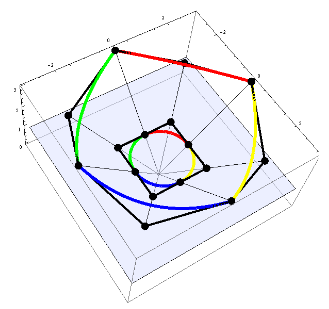
\includegraphics[width=6cm]{obrazky/NURBS-projection.png}
\end{center}
% Velikou výhodou NURBS křivek je právě schopnost zobrazit úplnou kružnici.
\end{frame}

\section{NURBS plochy}
\begin{frame}{NURBS plochy}
NURBS plochu získáme tenzorovým součinem dvou NURBS křivek.
\\\medskip
Výsledná plocha je pro řídící síť bodů $P_{i,j}$ s váhami $w_{i,j}$ kde $i=0,...,m;j=0,...,n$ a uzlové vektory $U=\left\lbrace u_0,...,u_k\right\rbrace$ a $V=\left\lbrace v_0,...,v_l\right\rbrace$ dána vztahem
$$S\left(u,v\right)=\frac{\sum_{i=0}^{m}\sum_{j=0}^{n}N_{i,p}\left(u\right)N_{j,q}\left(v\right)w_{i,j}P_{i,j}}{\sum_{i=0}^{m}\sum_{j=0}^{n}N_{i,p}\left(u\right)N_{j,q}\left(v\right)w_{i,j}}$$
\begin{center}
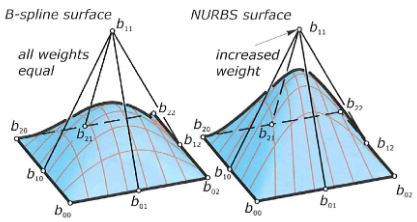
\includegraphics[width=7cm]{obrazky/nurbs-surface.png}
\end{center}
\end{frame}

\begin{frame}{Rotace}
Důležitou vlastností B-spline křivek je jejich afinní invariantnost - je jedno, jestli afinně transformujeme křivku nebo její řídící polygon, ze kterého potom vypočítáme transformovanou křivku
\\\medskip
\begin{block}{Rotace kolem osy $y$}
Afinní transformace vyjádřená vztahem $P^\prime=\vec{A}P$, kde
$$\vec{A}=\begin{pmatrix} \cos\theta & 0 & \sin\theta & 0 \\ 0 & 1 & 0 & 0 \\ -\sin\theta & 0 & \cos\theta & 0 \\ 0 & 0 & 0 & 1 \end{pmatrix}$$
Dostáváme
$$\begin{matrix} x^\prime=x\cos\theta+z\sin\theta; & y^\prime=y; & z^\prime=-x\sin\theta+z\cos\theta; & w^\prime=w \end{matrix}$$
\end{block}
\end{frame}

\begin{frame}{Zobrazení kružnice}
Mějme kontrolní body $P_0,...,P_8$ dle obrázku a jejich váhy $\begin{matrix}w_0=w_2=w_4=w_6=w_8=1; & w_1=w_3=w_5=w_7=\sin90^{\circ}=\sqrt{2}/2\end{matrix}$, pak pro uzlový vektor $U=\left\lbrace 0; 0; 0; \frac{1}{4}; \frac{1}{4}; \frac{1}{2}; \frac{1}{2}; \frac{3}{4}; \frac{3}{4}; 1; 1; 1\right\rbrace $ získáváme kružnici
\begin{center}
	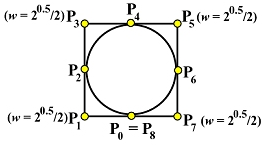
\includegraphics[width=7cm]{obrazky/circle.png}
\end{center}
\end{frame}

\section{Aplikace}
\begin{frame}{Aplikace}
Součástí této práce je aplikace v C\#.
\\\medskip
\begin{block}{Vstup}
Ve vstupním oknu uživatel zadá potřebné vstupní parametry: kontrolní body, jejich váhy, stupeň křivky, úhel rotace.
\begin{center}
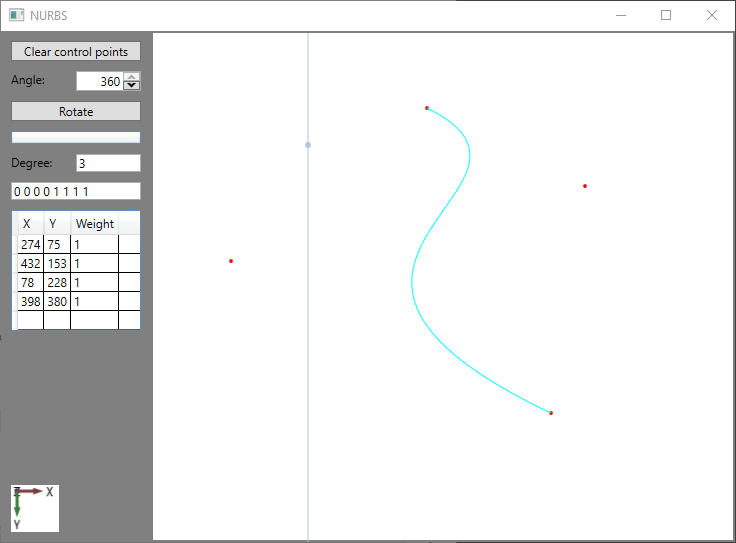
\includegraphics[width=6.8cm]{obrazky/screenshot-input.png}
\end{center}
\end{block}
\end{frame}

\begin{frame}
\begin{block}{Výstup}
Ve výstupním okně se uživateli zobrazí plocha vzniklá rotací kolem\\ osy $y$.
\begin{center}
	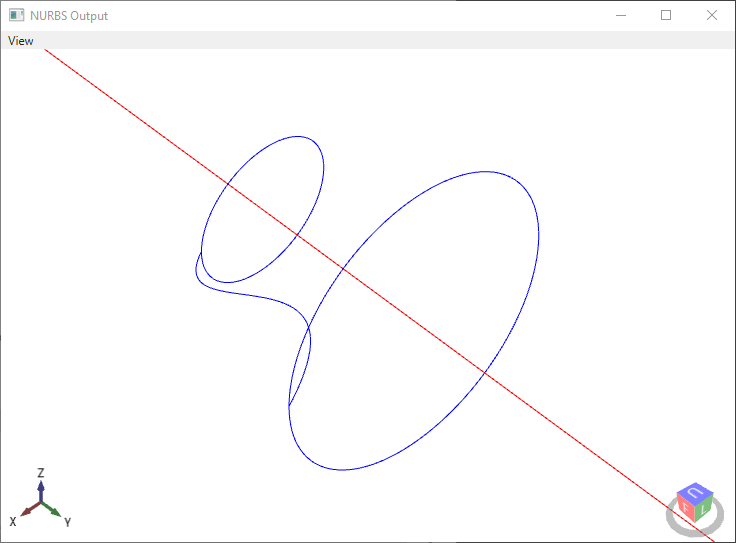
\includegraphics[width=8cm]{obrazky/screenshot-output.png}
\end{center}
\end{block}
\end{frame}

\appendix
\begin{frame}
	\begin{center}
		{\huge Děkuji za pozornost.
		\\\bigskip
		Dotazy?}
	\end{center}
\end{frame}

% \section{}
% \begin{frame}[containsverbatim]  %Pokud chceme použít prostředí verbatim
%   Základní syntaxe je následující:
%  \begin{verbatim}
% \section{Název sekce}
%    \subsection{Název podsekce}
%       \begin{frame}  %frame=slajd (tj. jedna stránka}
%          \frametitle{Titulek slajdu}
%          \begin{block}
%             Napis, který bude prostorově vystupovat
%          \end{block}
%          Nìco, co chci sdělit v jednotlivých položkách:
%          \begin{itemize}
%             \item $1+1=2$;
%             \item Něco důležitého;
%             \item A to nejlepší na konec.
%          \end{itemize}
%       \end{frame}
%  \end{verbatim}
% \end{frame}

% \subsection{}

% \begin{frame}
%  Ukázkový zdrojový kód této prezentace najdete na www stránce Ústavu matematiky

% \begin{center} {\tt http://www.math.fme.vutbr.cz}
% \end{center}

%  Odkazy
%         \begin{itemize}
%             \item Studijní obor Matematické in?enýrství
%             \item Informace pro studenty závìreèných
%  roèníkù. 
%             \end{itemize}
% \end{frame}

% \section{}

% \subsection{}

% \begin{frame}[containsverbatim]  %Pokud chceme pou?ít prostøedí verbatim
%   \frametitle{Práce s obrázkem}
%   V?echny obrázky by mìly být ve stejném formátu a pøeklad se dìlá
%   PdfLaTeXem (*.jpg, *.pdf)
%   nebo LaTeXem (*.eps, *.ps)
%  \begin{verbatim}
%   \begin{center}
%     \includegraphics[width=5cm]{krivitko.jpg}
%   \end{center}
%   \end{verbatim}
%  \begin{center}
%     %\includegraphics[width=5cm]{krivitko.jpg}
%   \end{center}
% \end{frame}


% \subsection{}
% \begin{frame}
%   \frametitle{Zajímavé zpestøení prezentace}
%   \begin{enumerate}
%     \item<1-> Bod 1. a 4. se objeví ihned.
%     \item<2-> Bod 2. a 3. je nejprve v pozadí.
%     \item<3-> Vystoupí do popøedí a? po stisku klávesy PageDown.
%     \item<1-> To je ten na první pohled viditelný bod 4.\qedhere
%   \end{enumerate}
%   \medskip
% \uncover<4->{A toto se zobrazí a? na ètvrté kliknutí :-)}
% \end{frame}


% \subsection{}

% \begin{frame}
%   \frametitle{Vlastní prezentace}
%   Prezentujeme vytvoøené PDF, které na celou plochu obrazovky
%   dostaneme pomocí CTRL+L (View/Full screen).
% \end{frame}


\end{document}
